\chapter{Autômatos finitos determinísticos}
\label{cap:afd}

No âmbito dos SEDs, um autômato finito determinístico (AFD) é uma máquina abstrata cujo funcionamento é descrito por uma dada carga de trabalho ordenada sequencialmente. Ao processar a informação de entrada, codificação sobre as operações requisitadas, o AFD acarreta duas possíveis circunstâncias: a operação corrente não é possível no estado atual da máquina -- e portanto o funcionamento é abortado -- ou toda operação é possível e feita. Nos dois casos, ao término, o estado do AFD é reiniciado. Além disso o único efeito interno das operações é a transição de estado, a quantidade de estados em que a máquina pode transitar é finita -- motivo pelo qual ela é denominada outrossim -- e ela não pode estar em mais de um estado simultaneamente, razão por que é determinística. O fato de os eventos, ou operações, ocorrerem em tempo discreto justifica sua modelagem nas teorias dos SEDs. O comportamento de vários desses sistemas pode ser modelado de forma simples, com AFDs.

Alguns estados dos AFDs podem ser marcados para algumas finalidades. Essas máquinas podem proporcionar formalismos reconhecedores de strings; é por isso que às vezes se refere às sequências de operações como palavras.

Haja vista que o presente trabalho objetiva especificar e demonstrar teoremas a respeito de AFDs, é indispensável definir essa classe de máquinas abstratas mediante formalismo. \citeonline{hopcroft} formulam AFD como uma quíntupla \begin{equation}\label{eq:afd_hopcroft}\langle Q, E, \delta, q_0, Q_m \rangle\end{equation} em que: \begin{itemize}
    \item $Q$ é seu conjunto finito não vazio de estados;
    \item $E$ é seu conjunto finito de eventos;
    \item $\delta : Q \times E \nrightarrow Q$ é a função que descreve as transições de estados;
    \item $q_0 \in Q$ é o estado inicial, a partir do qual a máquina inicia seu trabalho;
    \item $Q_m \subseteq Q$ é o conjunto de estados marcados.
\end{itemize}

A definição proposta por \citeonline{cassandras} inclui uma função de estados ativos $\Gamma : Q \rightarrow 2^E$ relacionando as operações possíveis a partir de um estado.

\section{Diagrama de estados}

Para auxiliar na visualização das transições entre os estados dos autômatos, os AFDs são comumente representados por diagramas de estados. Nessa representação, os estados são nós de uma estrutura semelhante a de grafos, e as transições, arestas que interligam dois nós, conforme a Figura \ref{fig:afd_diagrama}. Representam-se as transições cuja origem e destino são o mesmo estado por laços que partem de um nó e terminam no mesmo.

\figuradoautorantiga{Representação da transição no diagrama de estados}{
    \begin{tikzpicture}
        \node[state,minimum size=1.7cm] (q0) {$q$}; 
        \node[state,accepting,minimum size=1.7cm] at (4,0) (q1) {$\delta(q, e)$};
        \draw
        (q0) edge node{$e$} (q1);
    \end{tikzpicture}
}{fig:afd_diagrama}

Nessa classe de diagramas, os estados inicial e marcados podem ser destacados de alguma forma. Para este trabalho, uma seta sem nó de origem aponta sempre para o nó do estado inicial, e uma circunferência dupla enfatiza o de um estado final, como demonstra a Figura \ref{fig:afd_estado_inicial}.

\figuradoautorantiga{Representação de estados inicial (à esquerda) e marcado (à direita) no diagrama}{
    \begin{tikzpicture}
        \node[align=center,state,initial] (q0) {estado\\inicial};
        \node[align=center,state,accepting] at (4,0) (qf) {estado\\final};
    \end{tikzpicture}
}{fig:afd_estado_inicial}

Pode-se citar outros aspectos desta representação de autômatos: a possibilidade de adicionar rótulos aos nós, a opção de omitir os nomes dos estados nos nós quando não forem necessários e a aglutinação de transições que partem e terminam no mesmo estado em uma mesma aresta, com os símbolos separados por vírgula.

\section{Linguagens}

\section{Função de transição total e estado de ralo}

\section{Definição formal para Coq}

Embora amplamente aceitas, as definições matemáticas clássicas de AFD não podem ser diretamente aplicadas no assistente de provas Coq. Ele é, como explana o Capítulo \ref{cap:coq}, uma implementação de teoria de tipos; assim, é necessário que os elementos integrantes da definição tenham tipos. Ademais, implementações de teoria de conjuntos nessa plataforma não são triviais da forma que se apresentam na lógica interpretada por humanos. É incontrovertível deparar-se com a pergunta: como definir AFDs para estes propósitos e de modo correto?

À primeira vista mostra-se factível utilizar tipos indutivos em vez de implementar estruturas de dados para representar conjuntos. Sendo $\{ q_1, q_2, ..., q_k \}$ e $\{ e_1, e_2, ..., e_l \}$ os respectivos conjuntos de estados e eventos de um AFD, pode-se construir
\begin{equation}\text{\mintinline[escapeinside=!!,mathescape]{coq}{
Inductive Q : Type := q1 | q2 | !$...$! | qk.
}}\label{eq:Q_inductive}
\end{equation}
para os estados e
\begin{equation}\text{\mintinline[escapeinside=!!,mathescape]{coq}{
Inductive E : Type := e1 | e2 | !$...$! | el.
}}\label{eq:E_inductive}\end{equation}
para os eventos. Contudo, a fim de representar conjuntos finitos genéricos, essas construções não são possíveis. Representá-los como tipos quaisquer também não é sempre uma alternativa conveniente, já que isso permite instanciar tipos contendo infinitos elementos. A prova da decidibilidade de vários [citar exemplos] problemas acerca de AFDs baseia-se na finitude dos conjuntos de estados e eventos, evidenciando a importância de restringir tal atributo.



[Colocar opções que achei do StackOverflow]

Outra opção tange a especificar o recipiente dos estados na forma de lista e atribuir restrições a ela, fazendo o mesmo para os eventos. A biblioteca padrão de listas do Coq implementa uma coleção de funções, definições e notações que é útil para tanto. A implementação possibilita, por exemplo, uma notação semelhante à de pertence ($\in$) da teoria de conjuntos: \mintinline{coq}{In:forall X, X->list X->Prop}. A seguinte construção foi adotada:

\begin{minted}[escapeinside=!!]{coq}
Module Type AFD.
  Variables (A B : Type).
  Variable Q : list A.
  Variable E : list B.
  Variable transi!çã!o : A -> B -> A.
  Variable q0 : A.
  Variable Qm : list A.
  Variable ralo : A.
  Axiom transi!çã!o_correta : forall q e, transi!çã!o q e <> ralo -> In e E /\ In q Q /\ q <> ralo /\ In (transi!çã!o q e) Q.
  Axiom q0_correto : In q0 Q.
  Axiom Qm_correto : forall q, In q Qm -> In q Q.
  Axiom ralo_correto : In ralo Q /\ ralo <> q0.
End DFA.
\end{minted}

Restringir a decidibilidade das igualdades de \mintinline{coq}{A} e \mintinline{coq}{B} é importante no sentido de garantir as igualdades decidíveis dos AFDs\footnote{Os conjuntos de estados e eventos são finitos; logo, como aborda a Subseção \ref{ssec:eq_decidivel}, a igualdade entre seus elementos é decidível.} e permitir aplicar a proposição \mintinline[escapeinside=!!]{coq}{transi!çã!o_correta}, pois verificar se, para quaisquer elementos \mintinline{coq}{q:A} e \mintinline{coq}{e:B}, \mintinline[escapeinside=!!]{coq}{transi!çã!o q e} é igual ao estado de ralo requer $$\text{\mintinline{coq}{forall (a:A), {a = ralo} + {a <> ralo}}}$$ Mais, essa restrição facilita a prova de alguns dos lemas demonstrados pelo presente trabalho. Ela pode ser assim adicionada ao \mintinline{coq}{Module Type AFD}:

\begin{minted}[escapeinside=!!]{coq}
Axiom A_decid!í!vel : forall (x y:A), {x = y} + {x <> y}.
Axiom B_decid!í!vel : forall (x y:B), {x = y} + {x <> y}.
\end{minted}

A restrição não impede que qualquer AFD definido de acordo com a Equação \ref{eq:afd_hopcroft} seja escrito nesta formulação, porque os conjuntos de estados e eventos dos AFDs podem ser construídos com os tipos das Equações \ref{eq:Q_inductive} e \ref{eq:E_inductive}, inserindo todos os elementos dessas definições indutivas nas respectivas listas de estados e eventos. A igualdade é decidível para qualquer tipo definido conforme as Equações \ref{eq:Q_inductive} e \ref{eq:E_inductive}. A prova disso é feita por análise de casos da seguinte maneira:

\begin{minted}[escapeinside=!!]{coq}
Lemma Q_decid!í!vel : forall (x y:Q), {x = y} + {x <> y}.
Proof.
  destruct x, y; auto; right; intros; discriminate.
Qed.
\end{minted}

\noindent
cuja complexidade de tempo é $O(k^2)$, uma vez que a proposição é destruída em $k^2$ casos. Semelhantemente a complexidade para o tipo \mintinline{coq}{Inductive E} é $O(l^2)$. Em cada caso a tática \mintinline{coq}{auto} automaticamente prova a igualdade, e \mintinline{coq}{right; intros; discriminate} prova a diferença.

\section{Lemas úteis}

\subsection{Princípio da casa dos pombos}

\figuradoautor{Princípio da casa dos pombos}{
    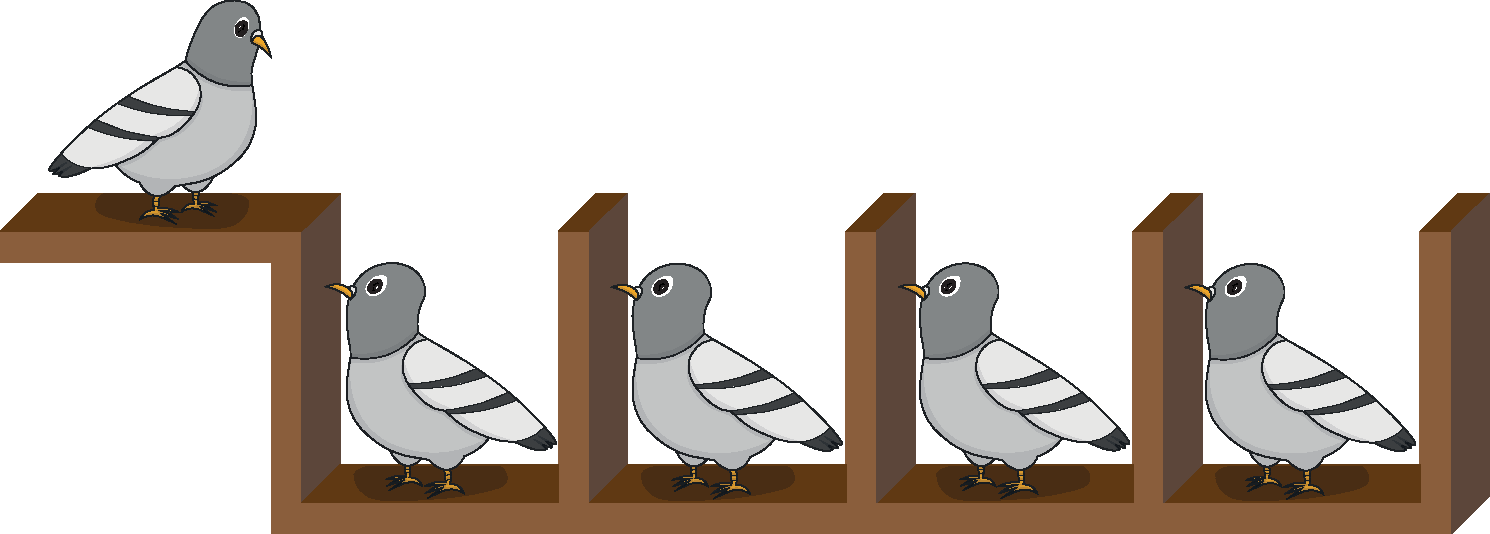
\includegraphics[width=.8 \textwidth]{imagens/pombos.pdf}
}{fig:afd_diagrama}

\begin{minted}{coq}
Lemma casa_dos_pombos : forall (l1 l2:A),
  (forall x, In x l1 -> In x l2) ->
  length l1 > length l2 ->
  repete l2.
\end{minted}

De acordo com \citeonline{jesper} e \citeonline{pierce}, a prova do lema \mintinline{coq}{casa_dos_pombos} não exige \begin{equation}\label{eq:InA_dec}\text{\mintinline{coq}{forall (a:A) l, {In a l} + {~ In a l}}}\end{equation} mas a demonstração de outra forma torna-se muito mais extensa. Para os propósitos deste trabalho, não obstante, o Coq tem, em sua biblioteca padrão, uma prova para a Equação \ref{eq:InA_dec} -- \mintinline{coq}{in_dec} -- sob a hipótese de que a igualdade de \mintinline{coq}{A} é decidível. Como a definição de AFD do presente trabalho restringe tal decidibilidade, a demonstração pode ser feita de modo trivial.

\subsection{Lema do bombeamento}
